\documentclass[conference]{IEEEtran}
\IEEEoverridecommandlockouts
% The preceding line is only needed to identify funding in the first footnote. If that is unneeded, please comment it out.
\usepackage{cite}
\usepackage{amsmath,amssymb,amsfonts}
\usepackage{algorithmic}
\usepackage{graphicx}
\usepackage{textcomp}
\usepackage{xcolor}
\usepackage{array}
\usepackage{xurl}
\usepackage{subfigure}

\usepackage{subfig}

\makeatletter
\newcommand{\linebreakand}{%
  \end{@IEEEauthorhalign}
  \hfill\mbox{}\par
  \mbox{}\hfill\begin{@IEEEauthorhalign}
}
\makeatother

% Define margins
\def\BibTeX{{\rm B\kern-.05em{\sc i\kern-.025em b}\kern-.08em
    T\kern-.1667em\lower.7ex\hbox{E}\kern-.125emX}}
    
% Define macros
\newcommand{\authorBlock}[6]
{
\IEEEauthorblockN{#1}
\IEEEauthorblockA{
#2 \\
College of Engineering \\
\it{Department of #3}\\
#4, #5 \\
#6}
}

% Document
\begin{document}


\title{BookMark - Bright Bookshelf}

\author{
\authorBlock{Mathilde Laerke Hansen}{9077620215}{Information Systems}{Copenhagen}{Denmark}{malaha@ruc.dk}
\and
\authorBlock{Sarah Schlegel}{9091820217}{Computer Science}{Paris}{France}{sschlegel@protonmail.ch}
\and
\authorBlock{Anais Zhang}{9088520214}{Computer Science}{Paris}{France}{anais.zhang12@gmail.com}
  \linebreakand 
\authorBlock{Young Ha}{2017029261}{Information Systems}{Seoul}{South Korea}{dudgk970@gmail.com} 
\and
\authorBlock{Laura Vikke Martensson}{9077020219}{Computer Science}{Copenhagen}{Denmark}{lauramaartensson@gmail.com}
}




\maketitle

\begin{abstract}
Nowadays, modern people (employees, students, etc.) lack time for reading books. Although they have the motivation to read, when people are investing time in various activities such as studying, working, or exercising, the time for reading has low priority amongst the 24 hours of a day. For example, even if you want to read a book, the hardships of choosing and purchasing a book yourself are an obstacle to reading. \\
To meet the aspiration of overcoming these obstacles, we created the application BookMark. BookMark is meant to help the customers manage their bookshelf, either physical or digital, and arrange more time in their daily life to read. BookMark provides a system of reminders to keep track of the books the user is currently reading, and makes the bookshelf management easier by using simple image recognition to search for a book by its cover, barcode, or ISBN number. It automatically sorts the content and providing different pairing options between physical copies, ebooks or audiobooks. By automatizing the usually difficult part of book management, BookMark wishes to let the reader make more space in his or her day to actually read.
\end{abstract}


\subsection*{Role Assignments}

\begin{center}
\begin{tabular}{ | m{1.8cm} | m{1.5cm}| m{4.2cm} | } 
 \hline
 Roles & Names & Task description etc. \\ 
 \hline
 User / Customer  & Young Ha Hwang & Ordinary people fitting in to modern society are main users of the application. We assume that they are willing to read, but that reading priorities are set low due to other activities. To check the sustainability of the application, first, a simple survey was conducted to determine users' time management for reading, if they are currently reading a book and how reading is prioritised in their everyday life. \\ 
 \hline
\end{tabular}
\end{center}

\begin{center}
\begin{tabular}{ | m{1.8cm} | m{1.5cm}| m{4.2cm} | } 

 \hline
 Project manager & Sarah Schlegel & The project manager is in charge of planning, assigning the tasks and is generally in charge of ensuring that the project is moving forward. She will make sure that the team meets the different goals at the right time. She has the responsibility to inform the development manager of any changes regarding the project requirements. \\
  \hline
  Development manager &  Mathilde Lærke Hansen & The development manager confirms the final functions of the software with considerations of the user as the main consumer of the application. The development manager mediates and updates the software developers. If the software does not live up to the users needs and expectations, the development manager will gather more information about the customers and then advise the software developers how to fulfill the needs of the user.\\
  \hline
 Software developer & Anais Zhang \&  Laura Vikke Mårtensson & The software developers reflect on which software system that would fit the best for the application. They analyze, categorize and examine the software and make decisions of which development tools that can be used to implement the applications. They collaborate with the development manager \\ 
 \hline
\end{tabular}
\end{center}



\section{Introduction}

\subsection*{Motivation}
The idea for the BookMark project derives from an observation that many people today don't have the time nor the motivation to read new books as they navigate their fast paced and overstimulated everyday life. Our goal is to provide, with this combination of a bright bookshelf and mobile BookMark application, a simpler way to manage the books people are reading, whether it's by swapping from a physical book to an audio book, by reminding the user to read at certain times or by recommending them new books based on their current preferences. \\ \\


This application focuses on making reading more efficient for people and helping them sort and keep track of their books on a physical bookshelf. There is no time in the schedule of most people to read books that are not academic or work related. Also, people who actually manage to find the time to read usually keep a physical bookshelf. On the other hand they could keep a list of audiobooks and ebooks on their devices, and have their bookshelf right in their pockets or keep both physical and mobile. For peoples who have a lot on their plates, sometimes they might forget their physical copy at home, or maybe want to do a task while listening to their book. Maybe it would help them to have the ebook and the physical copy, and they'd like to switch from one to the other easily without struggling to find the correct page between the different versions.\\
BookMark is meant to help with these issues mentioned above. If the users can keep track of their reading, and get reminders of their current position in a book, they can be more eager to pick up their book again. BookMark will help the user put the book back to the correct place in a physical bookshelf and not organize a personalized sorting system. When they're done reading and have to get going, they just have to note their current position in the book in the app, whether it's the chapter or the page they left it, and they won't lose track of their progress in the book. \\ \\

Furthermore, if they have already purchased the physical copy, they can simply scan the barcode, the ISBN number, or even just the cover, and the app will give the user alternative options like if the book is available as an audiobook or an ebook, so that they can read or listen as they prefer. The app will also propose time slots to read when a person has a break in their calendar and propose new books they may like to read next, so that they don’t have to search for books that they might like. The application will get to know the user, and therefore know their likes and dislikes. If they purchase an ebook or an audiobook copy, they can directly start listening to the audiobook or reading the e-book on their phone. This application is available through a simple sign up phase and afterwards the subscriber has their own personal login. A chat feature will also be available as a help to the user if needed. The ambition of BookMark is to assist people with their busy schedule and provide space to read more books at their desired pace.

\subsection*{Problem Statement (client's needs)}
Through a questionnaire, we found out, as suspected, that students feel that they do not have the time to read books in their everyday life. We asked different people questions about their normal life. The biggest feedback from an age group was people between 15-26 (94\%). We asked what they need more of in their life, and the number one answer was: time. Other top answers were money and love.\\
The reasons for reading amongst the questioned people were to learn, for entertainment, or for relaxation. To the question: “What would make you read more books?” The answer “more time” was the most frequent one, but here are some other answers worth mentioning: “more awareness of the books out there (too many to know them all)”, “if finding interesting books didn’t require so much research”, “Easier way to get physical books” or “A better variety of English ones in store”.\\
The testet people usually either read 30 minutes before bed, in the summer vacation (when there is no school or work) or during commute on their phones or with a physical book. Some of them have experience with using audiobooks, but most of them don't. The ones that do listen to audiobooks, do it so that they can do other things at the same time.\\
The survey is only a sample test and we acknowledge that this questionnaire is only a snapshot of reality. We only use the stats as an inspiration for our different features in our application.


\subsection*{Research on any related software}
There are quite a few concepts already on the market, or in progress of development, that resemble online bookshelves or ways to track your reading progress. These range from large physical bookshelves aimed at libraries as the targeted consumer, down to mobile applications which help you to keep track of the books that you are reading or want to read.
\begin{itemize}
	\item RFID smart bookshelf
	\item Smart AI Modular Bookshelf
	\item Goodreads
	\item BookBrowse
	\item StoryGraph
\end{itemize}


\subsection{RFID smart bookshelves} 
This company produces large smart bookshelves that are designed to be used in a library and make work for the employees easier. The bookshelves communicate with a central file management system and works by scanning books in real-time through an antenna array. The system has useful functions such as; easy navigation to books when looked up in the system, generating reports when books are placed on the wrong shelf by a reader or an employee and detecting missing books. These bookshelves and their associated functions are very useful and mostly designed for the needs of huge libraries and professionals who are handling a lot of books. In contrast, our project focuses more on the needs of the private consumer, and is designed to help the individual reader with managing their private book collection.\cite{RFID} \\

\subsection{Smart AI Modular Bookshelf} 
This is a concept developed as a way to help the private book owner to better manage their books. It is a physical smart bookshelf connected to an application, which is then used to manage the book collection. The bookshelf uses image recognition technology to keep track of the books location, and embedded lightbulbs in the bookshelf will light up when searching for a specific book. The application offers functions such as reading project management and book reviews. This product is, at this point in time, only a concept and not an actual product on the market. Our project expands on the idea with additional functionalities and features.\cite{Smartbookshelf}\\

\subsection{Goodreads} 
Goodreads is a website and an application, which is meant to keep track of the books that you’re reading, have read and want to read. The main functionalities of Goodreads are meant to help the user to choose a book to read, with features such as book reviews, personalized book recommendations and insight into what your friends and the rest of the Goodreads community is reading. \cite{Goodreads}\\

\subsection{BookBrowse} 
BookBrowse is a book recommendation website who offers excerpts of books to skim just as you would when you browse for books in a library. You can also find Independent and in-depth book reviews, as well as personalized book recommendation and a bookclub subscription. \cite{Bookbrowse}\\

\subsection{StoryGraph} 
This application offers you personalised book recommendations, as well as tools to keep track of your reading progress and statistics. If you have a Goodreads account, you can import your data into the application. \cite{Storygraph} \\

\section{Requirement Analysis}

\subsection{Log-in}
When the user download the app, the main page shows two inputs for the email and password to sign in if the user already have an account. If they don't have an account, they can create one with the \textit{Create} button below the login form on the main page, which will redirect them to the sign up page. Finally, a smaller link can lead them to the account recovery page in case they forgot their password.\\
For the login process, the software looks into the database to find the matching combination of username and password or email and password for a user. After logging in, the user is redirected to his main page, \textit{My BookMark}.\\

\subsection{Sign up}
Membership requires basic information such as a unique username, a valid email, a password, and an optional phone number for password recovery. The password has to be at least 8 characters long, with one uppercase, one lowercase, one number and one symbol.\\
The app also requires the user to agree with the terms and conditions, and optionally to subscribe to the newsletter. The terms and conditions are displayed in a scrollable pop-up that allows the users to read them without losing the data they've already input in the form.\\
The sign up process then creates a 8-digit token and sends it to the user in a confirmation email, in clear and in a hyperlink. The hyperlink leads to a confirmation page that will display the success of the confirmation.\\
Once the email has been verified, the user can log into the app. For the first connection, the user must choose at least 3 genres of books he or she likes to set as reading preferences for the recommendation algorithm.\\


\subsection{My BookMark}
The home page of the app functions as a 'hub' from where you can access all the different features of the application. The bottom menu is composed of five buttons, each represented as a symbol:
\begin{itemize}
	\item Home: brings the user back to the home page
	\item Library: takes the user to the list of books (\textit{My Bookshelf} page)
	\item Add: goes to \textit{Add a book} page
	\item Statistics: brings the user to his \textit{Statistics} page
	\item Account: goes to the \textit{User account} management and settings page
\end{itemize}

The home page in itself consists of a preview of the user's shelves and categories. By clicking on each element, the user opens a more detailed page of the shelf or category, listing all the books that it's referencing and his current progress in those books. When he clicks on one of them, he triggers the \textit{Book view}.\\

\subsubsection{Add a book}\hfill\\

The user clicks the central + button in the bottom menu to add a new book. This action displays a pop-up to ask him if he wants to enter the book manually or use the camera to scan the book's cover, the ISBN number or the barcode.\\
If he selects the scan option, the app opens the camera and the user scans the book. If it's the cover, the image is decomposed using an image recognition library to figure out the book title and pair it with a book in the user's collection or a book in the internet databases. If it's a barcode or an ISBN number, the app searches in external APIs to find the book reference through the given number. Once the app has found a matching book by image recognition or by an external request, it asks the user to confirm that it's the correct book and if he wants to add this book to his library. If yes, the book is added to the library and assigned to a shelf on the bookshelf. The shelf lights up to show the placing of the book.\\
If the user has selected the manual entry of the book, he is prompted to enter the book title and author. The book is then searched on the Internet and the ISBN and book title are displayed to the user to ask him if it's the correct book and if he wants to add it. Then we repeat the same process as for the scan option to assign the book to a shelf.\\

\subsubsection{My Bookshelf}\hfill\\

This page displays a list of the books and ebooks owned by the user sorted depending, listing them in different categories:
\begin{itemize}
	\item New Arrivals: shows the two most recently added books.
	\item Currently reading…: shows the books the user is currently reading, sorted by latest reading update.
	\item Wishlist: shows the books the user has added to his wishlist from the recommendations.
	\item Recommended: recommended books depending on what the user has already read. Clicking on this list redirects to the \textit{Suggested books} page.
	\item All books: displays a list of all the books depending on the user's sorting parameters (author, title, genre). The sorting type can be selected in the \textit{User account} settings.
\end{itemize}
Each category at first only displays 4 books, but it can be expanded to display the complete list.\\
The page also has a search bar to find a book easily. When the user starts inputing text in the search bar, the app searches for the book depending on the title or author's name in the user's bookshelf, hiding the rest of the categories. If the book isn't in the user's bookshelf, the search shows 'No results' and proposes to search for the book on the Internet and in the book database.\\
By clicking on a book, the user toggles the \textit{Book view} for this specific book.\\


\subsubsection{Book view}\hfill\\

The book view displays the book data: title, author, eventual number of pages, shelf position, current labels, reading status and notes. If he clicks on a little bookshelf icon atop of the page of a book of which he owns a physical copy, the physical bookshelf will light up the shelf on which the book should be stored, depending on the current sorting parameters.\\
The user can update the following things on the book:\\
\begin{itemize}
	\item The label assigned to the book (read, not read, currently reading);
	\item His reading status (current page or chapter number);
	\item His personal annotations, whether they're global or whether they are related to a specific page or chapter;
	\item His personal rating, with zero to five stars;
	\item Specific reminders to read this book if he's currently reading it.
\end{itemize}

If the user wants to remove the book from his app library and from his bookshelf, he can click on a button at the bottom of the Book view. A popup window will appear to ask him if he's certain to want to remove this book from the bookshelf and from the library. The book will then be removed from the user's collection and from the positioning in the physical bookshelf.\\

\subsubsection{Suggested books}\hfill\\

A separate page displays the recommended books for the user depending on the books he already owns. For this, we will design a personal machine learning algorithm inspired by popular suggestion algorithms like Netflix's, YouTube's, Instagram's or Amazon's.\\
The page consists of a list of books and covers. If the user clicks on a book, it will toggle a simplified book view with the title, author, number of pages, and a + button to add the book to his bookshelf.\\

\subsubsection{Statistics}\hfill\\

The statistics page displays information about the user's reading history and bookshelf data in the form of graphs and numbers. The statistics displayed are the following:
\begin{itemize}
    \item Last books read: The names and links to the 3 books that were updated the most recently, whetter read or currently reading.
    \item Graph of books read: A bar chart displaying the number of books read in the last 3 months.
    \item Bookshelf completion: The number of books read over the total number of books in the bookshelf.
\end{itemize}
That way, the user can keep track of his current progress.

\subsection{Physical Bookshelf}

The physical bookshelf comes in various sizes and colors, but in a common simple design that appeals to many different types of people. The bookshelf will need to be plugged into a power source in order to function and be able to connect with the associated app. On each shelf there is a LED band that can light up when triggered by the app.\\

\subsubsection{Connect to bookshelf}\hfill\\
In the user settings, there's an option titled 'Bookshelf' to configure the user's physical bookshelf.\\
If the user is not yet connected to the bookshelf, when he selects this option, a large pop-up appears. If the Bluetooth is off, it asks the user to turn off the Bluetooth. When the Bluetooth is on, it starts searching for devices ready for connection, and displays only the nearby BookMark bookshelves. If the user clicks on one of them, it prompts him for a connection confirmation. Multiple users can be connected to the same bookshelf.\\
Once the user's account is bound to the physical bookshelf, when the user clicks on the Bookshelf option in the settings, the page displays the informations of the bookshelf. These include the id number, the dimensions, the number of shelves, the number of books in the bookshelf, the number of audiobooks and ebooks and the sorting and sub-sorting categories.\\
The sorting categories are two dropdowns that allows the user to select between sorting by title, author, genre or none. If the user changes the sorting category, a pop up is displayed to confirm the change and recompute all the sorting in the bookshelves. page will display a graphical preview of the bookshelf and all the books in the right order.\\

\subsubsection{Disconnect from bookshelf}\hfill\\
At the bottom of the bookshelf information page, there's a button to disconnect from the physical bookshelf. If the user clicks it, it prompts him for confirmation in a pop up window. When the user disconnects from the bookshelf, the books on his account are preserved but the shelving and the sorting in the bookshelf are deleted.\\
If the user is the only user connected to the bookshelf, the app asks him if he also wants to delete all the bookshelf recordings. If he does, all the related data to this bookshelf in the database will be dumped.\\

\subsubsection{Book lookup}\hfill\\
When the user scans a book that is already in his collection or selects a book from the list on the app, the smart bookshelf lights up the correct shelf to highlight the correct position of the book depending on sorting. Or, the other way around, the user can select a book in the app and click on a button and it will light up the shelf on which the book should be stored.\\

\subsubsection{Bookshelf sorting}\hfill\\
In his settings, the user can view the current sorting of the shelves in two dropdowns: sorting and sub-sorting. If none is selected, the books are just stored by date added. If a sorting (by genre, author, title, etc.) is selected, then in the All Books category of \textit{MyBookmark}, the book previews will be rearranged depending the sorting category.\\
By clicking on a shelf or in the sorting menu in \textit{MyBookmark}, the user can rearrange the bookshelf sorting manually or select a new sorting category. \\
If he wants an automated sorting, he selects the main sorting category (genre, author, title, etc.) and the app will compute the best rearrangement of the books depending on the books available in physical copies, the main sorting category and eventually another sub-sorting option (sort by author then book title for example).\\
If he wants to sort them manually, he can move the books from shelf to shelf by clicking on a button or drag-and-dropping them from shelf list to shelf list.\\


\subsection{Settings}\hfill

In the settings page, the user can change the language of the app, or change the mode of his screen (dark or light mode) and set all the reading notifications. A switch will be available for the user if he wants to activate or deactivate reading notifications is activated by default.\\

\subsubsection{User account}

In the user’s account page, the user can check his personal information like his username, phone number or email. He can also change these informations.\\
To change his email, the app requires the user to enter his password. If he changes his email, it will trigger the sending of a confirmation email to the new email; until then, the new email will not be used.\\
For changing his password the users must put his current password and then the new password twice to confirm the newest one. As for the signup, the new password must be  at least 8 characters long, with one uppercase, one lowercase, one number and one symbol.\\

\subsubsection{Account delete}\hfill\\
At the bottom of the account page, there's a button for deleting the account. Clicking on that button toggles a confirmation popup to ensure the user really wants to delete his account. Then, the user has to click the link received in a confirmation email to terminate his account. His preferences, informations and data stored will be deleted from the database and the physical bookshelf will be unbound from the user's account.\\

\subsubsection{Reading frequency}\hfill

The user can change his reading frequency with 2 possibilities: per day or per week.\\
There is a button to let the user choose his frequency of reading.\\
If a user chooses to read every day he must specify the hour that he would like to read.\\
If a user chooses to read every specific day in a week he must choose which days and time he wants to read.\\
According to his choice a pop up will appear to help users to select time or date and time.\\
Default setting for reading time is automatically set every day at 9am.\\

\subsubsection{Log out}\hfill\\
The logout button at the bottom of the user's settings list. To log out users just clicks on the button and a pop up appears to confirm the log out. The user is redirected back to the \textit{Log in} page.\\


\subsection{Audiobook/Ebook binding}
In his personal account, the user can bind his Amazon, Kindle, Audible or other reading accounts to sync his libraries.\\
When his libraries are synced, the user can toggle the opening of another app (Kindle, Audible, etc.) to jump directly to the audiobook or ebook depending on his current position:\\
For an audiobook, it plays the audiobook from the saved timestamp\\
For the ebook, it opens to the correct page in the reading app.\\


\section{Development Environment} 
\subsection{Choice of software development platform}

Our development environment will be mostly UNIX based and Apple oriented since most of us have Apple products such as iPhones or MacBooks. That way, we can use tools that are already provided in the Apple development environment, such as the Xcode IDE. Xcode is created by Apple and therefore optimized to create application for OS devices, with the possibility to run the app on a simulator or on a connected iPhone to see the progress, and it comes with built-in tools for iOS and MacOS development.\\
The code and documentation will be held on a public GitHub repository to grant easy access and have a good overview of the project progress.\\ 

\begin{center}
\begin{tabular}{ | m{1.9cm} | m{5.7cm}| } 

\hline
Tool/language & Reasoning \\
 \hline
 Swift 5.5 &  Swift is a programming language created by Apple inc. in 2014 and is designed to be powerful and intuitive when writing code and applications for Apple OS devices. It has an intuitive syntax, close to C-based languages, and it can be used in combination with Xcode to preview the application interface while it is developed. We will use this language to create the front-end of the application with the default 5.5 version which is included in Xcode.\\
  \hline
 OVH VPS (Apache) &  The server is be a Virtual Private Server hosted on by OVH. It is configured with a Debian 10 OS, and Apache 2 for web hosting, and has basic access as well as a root access for doing all the configuration. The MySQL database is set up directly on the server.\\ 
 \hline
 MySQL & We need a database to manage the data related to books, users and bookshelves. MySQL is an open-source database management system, widely used and popular for handling small and big databases, easily installed on a server and is used in combination with the SQL language in order to manage the data.\\
 \hline
 \end{tabular}
 
 \begin{tabular}{ | m{1.9cm} | m{5.7cm}| } 
 \hline
 PHP/JS & The backend website for management, whether it's users, books or bookshelves, will be in PHP and JS. PHP is the most common scripting language for web development, along with JavaScript, and the combination of both allow for a fast website with asynchronous queries and dynamic updates. We will especially be using JQuery to simplify the JavaScript syntax.\\
 \hline
 Python & Python is a high-level general-purpose programming language which supports both object-oriented and functional programming. Many public Python libraries focused on machine learning and AI are available, which is why we chose this language to create the AI part of our project. \\
 \hline
 C++ & C++ is a middle-level, compiled and object-orientated programming language. As we will be running the database for the application on a server, it is easier to have a middle to low level language for the API since the execution speed will be higher. Also, C++ has known libraries for API management which will simplify the API construction.\\
 \hline
 
\end{tabular}
\end{center}
\hfill

\subsection{Cost Estimation}
\hfill

\begin{center}
\begin{tabular}{ | m{4.6cm} | m{3cm}| } 

\hline
Resource & Price (Won) \\
 \hline
 Web Server  & 23.571 \\
 \hline
 Apple Developer License & 116.676 \\
 \hline
 
\end{tabular}
\end{center}

\hfill
\subsection{Software in use}
\subsubsection{Goodreads}\hfill\\

Goodreads has an application on the market that includes some of the same functionalities as our project, but does not offer the option to connect with a physical bookshelf. Goodreads has a section called 'My Books', as seen in Figure \ref{fig:goodreads} which is designed to keep track of the books in the users collection, and offers the option to use the camera to scan the physical books in your collection. BookMark will offer a similar book management system, but will be synchronized with the users books placement in the physical bookshelf to create an even more powerful organizing tool for the user. \\


\begin{figure}[h]
    \centering
    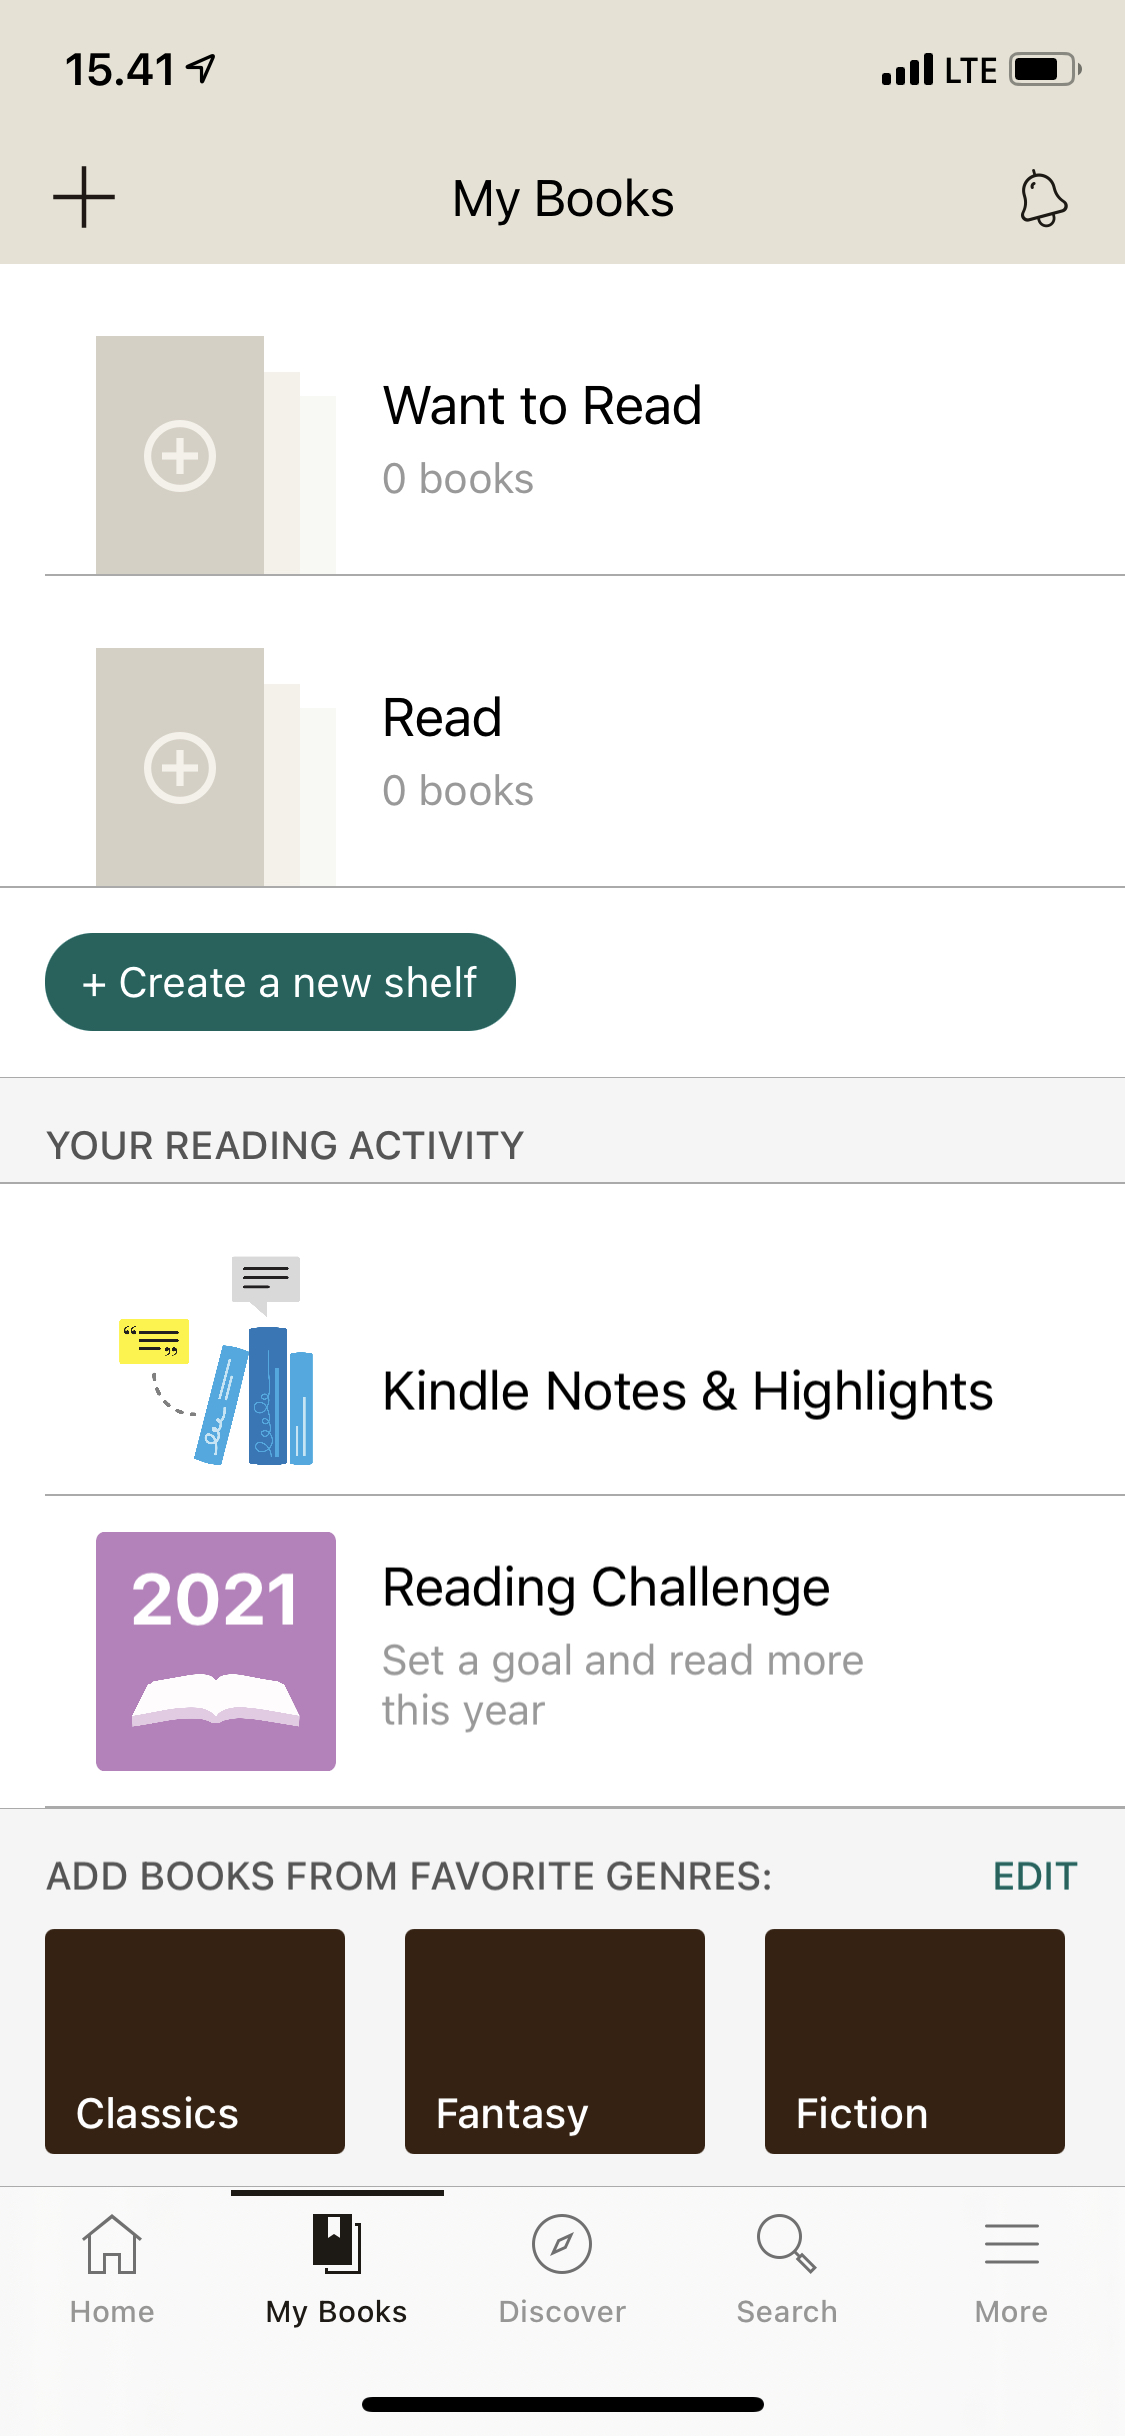
\includegraphics[width=3cm]{Ressources/Software in use/goodreads.jpeg}
    \caption{Goodreads app: My Books}
    \label{fig:goodreads}
\end{figure}

\subsubsection{Amazon API}\hfill\\

The application offers the functionality of 'Add a book' to the user's virtual bookshelf, which requires the app to be able to access some sort of database of books. For this purpose, BookMark will make use of an Amazon Books API for searching and looking up books available in Amazon. For the scope of this project, Amazon currently offers free access to a HTTP or REST API, which can be accessed with the help of a Lambda function for the backend. \\
  

\subsection{Task Distribution}
\hfill

%(If you want, you can provide this later at the nextphase-design)
%       Which member is responsible for what? 

\begin{center}
\begin{tabular}{ | m{3.5cm} | m{4.1cm}| } 

\hline
Name & Responsibilities \\
 \hline
 Sarah Schegel  & ? \\
 \hline
 Mathilde Lærke Hansen & ? \\
 \hline
 Young Ha Hwang & ? \\
 \hline
 Anais Zhang & ? \\
 \hline
 Laura Vikke Mårtensson & ? \\
 \hline
 
\end{tabular}
\end{center}

\section{Specifications}

\subsection{Database}

\begin{figure}[h]
    \centering
    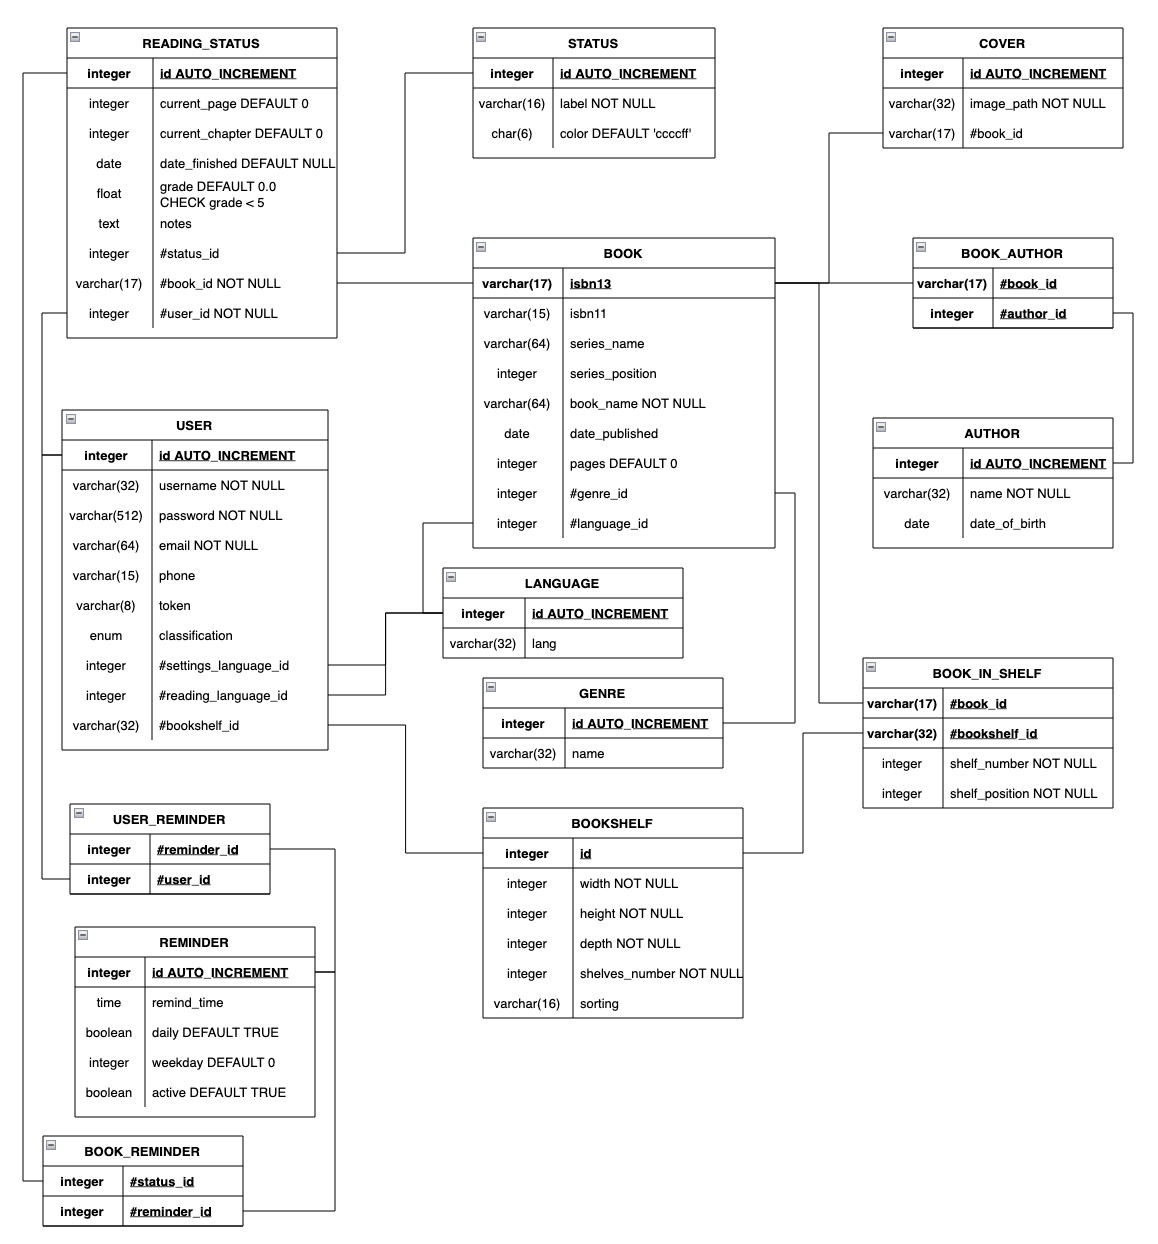
\includegraphics[width=9cm]{Ressources/Specifications/LDM.png}
    \caption{Logical Data Model\cite{LDM}}
    \label{fig:ldm}
\end{figure}

Figure \ref{fig:ldm} shows the Logical Data Model of the database. The primary keys of the tables are in bold, the types of the columns are on the left side and the names and constraints (check values and default values) of the columns are on the right side. The foreign keys are identified with a \# and linked to the table they are referencing.
The main tables of our database are the 'user', 'book', 'bookshelf' and 'reading\_status'. Along with the associative tables and the other tables for satellite data, these four tables are the ones that will be used the most for managing our users and our bookshelves.

\subsection{Log-in}

The Log-in page as shown in figure \ref{fig:login} is the first page that the user will be met with when they have downloaded the application and opened it for the first time. The user will have to input username and password using the mobile keyboard, and the application will (use API?) to request the database if such a user exist, when the user presses 'Log-in'. If in existence in the database, the user will be guided to the home page, e.g 'My Bookmark'. If the user does not already have an account, a button called 'create' is displayed in the bottom of the screen, which will guide the user to the sign-up page. Lastly, if the user has forgotten their password, they have the option to request a new password from the log-in page.

\begin{figure}[h]
    \centering
    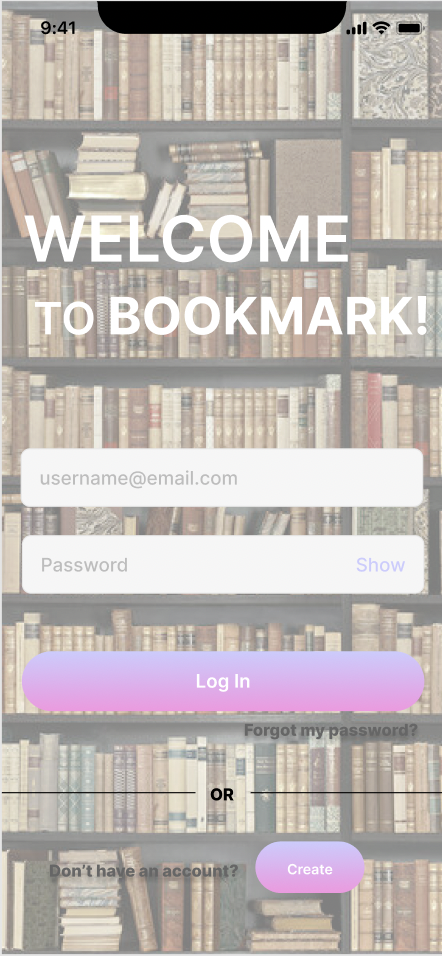
\includegraphics[width=3cm]{Ressources/Specifications/Login.png}
    \caption{Log-in page}
    \label{fig:login}
\end{figure}

\subsection{Sign-up}
If the user does not already have an account and have therefore been guided to the sign-up page, as seen in Figure \ref{fig:signup} there are several datapoints that the user will have to input in order to be created in the database. An username, Email, Phone number and sufficiently secure password should be inputted. Moreover, the user has to agree to the terms and conditions of the applications, of which can be accessed and read through a hyperlink. Lastly, the user has the opportunity to sign up for a newsletter, where they will be registered in a mailing list and send regular emails with personalized book recommendations and etc. based on their data. \\
After the user's sign-up details has been approved and created in the database, the user will be guided to a new page, as seen in Figure \ref{fig:categories} where they have the option to choose their favorite genres such that the recommendations and search results in the app will become more relevant to the users personal preferences. 


\begin{figure}[h]
    \centering
    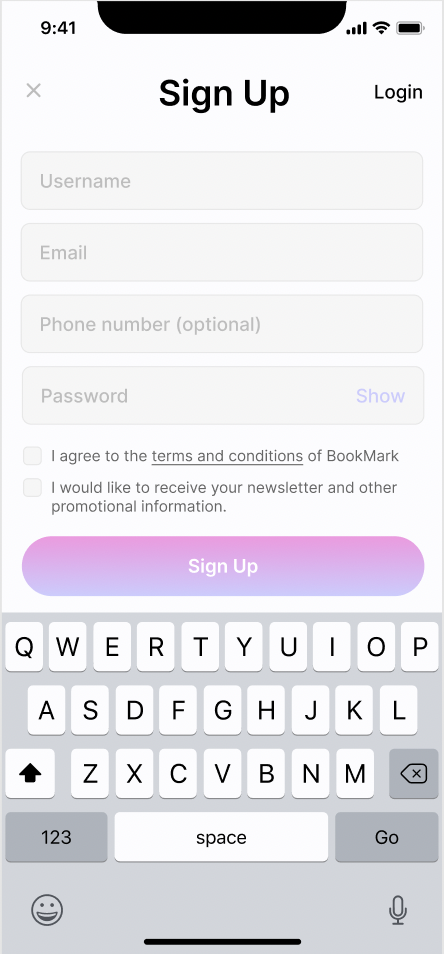
\includegraphics[width=3cm]{Ressources/Specifications/signup.png}
    \caption{Sign-up page}
    \label{fig:signup}
\end{figure}

\begin{figure}[h]
    \centering
    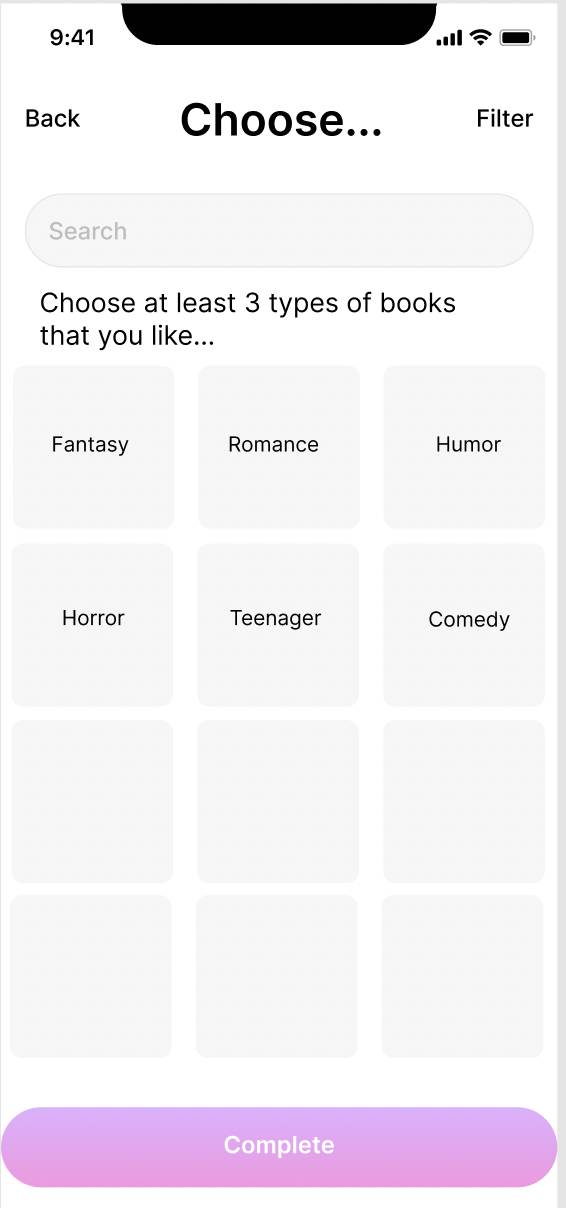
\includegraphics[width=3cm]{Ressources/Specifications/categories.png}
    \caption{Preferences page}
    \label{fig:categories}
\end{figure}



\subsection{My BookMark}
The page 'My BookMark', as seen in Figure \ref{fig:mybookmark} is the first page the user will be guided to when they are already logged in and opens the app. It is the user's personal page where they will have the option to upload a photo of themselves in order to personalize their page, and they will be able to access different main functionalities of the app. At the top of the page, the user will have the option to press a 'back' button, which will guide them to xxxx, and a '+' button which will guide the user to the 'Add a book' page. \\

'My Bookmark' will also preview of the user's current bookshelf with images of the bookcovers. They will have the option to view all the books in their collection from the the default 'My books' view, as well as a views called 'Now reading' which will provide different options if clicked on a book, as seen in Figure \ref{fig:book}. The user will be able to see their reading progress, rank the book, delete the book from their collection and keep reading the book. If the user chooses to 'Keep reading' the book will either be opened as an Ebook, or the physical bookshelf will light up where the pysical book is stored.  \\

At the bottom of the page, which will be available from most pages within the application, the user has access to the four main sections of the application, as well as a '+' button for quick access to adding a new book to the user's collection. The first button will guide the user to the main page, the next to the 'My Bookmark' page, the third to the reading statistics page, and the last to the 'User Account' page.

\begin{figure}[h]
    \centering
    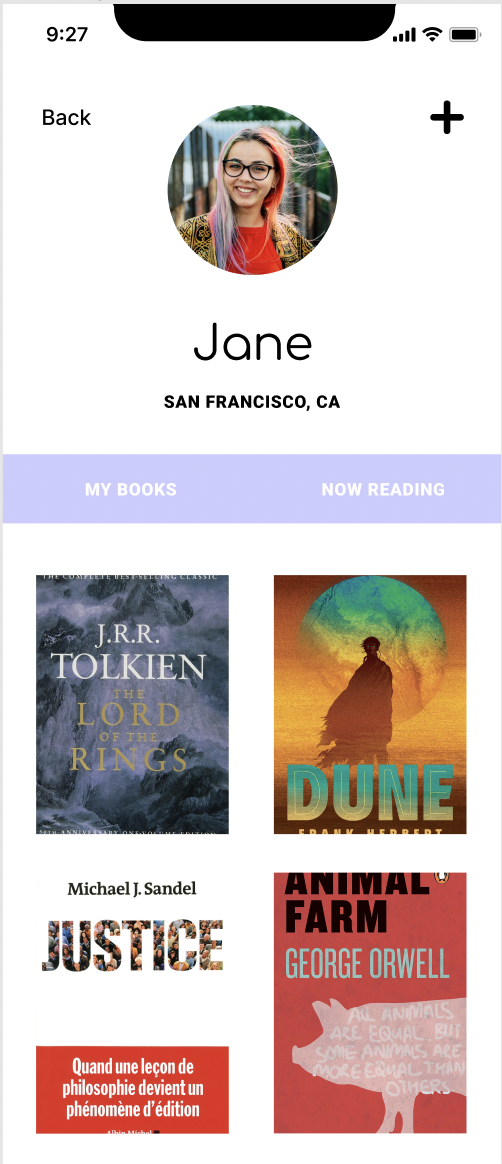
\includegraphics[width=3cm]{Ressources/Specifications/mybookmark.png}
    \caption{My Bookmark page}
    \label{fig:mybookmark}
\end{figure}

\begin{figure}[h]
    \centering
    
\includegraphics[width=3cm]{Ressources/Specifications/book.png}
    \caption{My Book page}
    \label{fig:book}
\end{figure}

\subsection{Add a book}
When the user press a '+' button anywhere in the app, they will be met with a pop-up asking if they wish to add a physical book or an ebook. If they choose ebook, they will be be shown a 'search' page which will show updated suggestions based on what the user inputs in the search field. When the user has located the book they want to add, they will be guided to the 'Add a book' page, as seen in Figure \ref{fig:addabook}. \\
This page previews information about the book, as well as ratings and reviews from other users of the application. The user will press the button 'Add My List' to add the book to their bookshelf in My Bookmark.\\

If the user chooses to add a physical book, they will be guided to a new page using the camera in order to be able to scan the cover, ISBN or barcode of the book. Then the book is automatically added to the user's bookshelf in My Bookmark, and the physical bookshelf is updated to recognize this book as a part of its collection as well.

\begin{figure}[h]
    \centering
    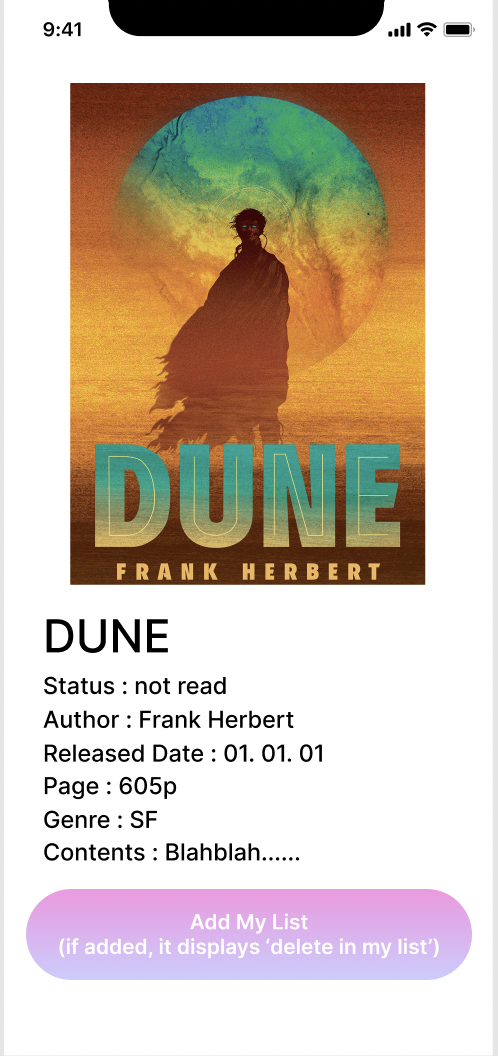
\includegraphics[width=3cm]{Ressources/Specifications/addabook.png}
    \caption{Add a book page}
    \label{fig:addabook}
\end{figure}

\subsection{Main page}
The main page, as seen in Figure \ref{fig:mainpage}, functions as a mixture between an overview and a discover page, where the user will be able to view the books they are currently reading as well as discover new books, which the application suggests based on personal preferences. There will be recommended books based on the user's preferred genres, books similar to the one the user has already read and New Arrivals which fits the user's preferences. \\

The user will also have access to a search function they can use based on book names and authors, which will search the database for the requested book or books.\\
At the top left of the page, the user user will have the opportunity to to log-out of the application and at the top right the '+' button us present, guiding the user to the 'Add a book' page.

\begin{figure}[h]
    \centering
    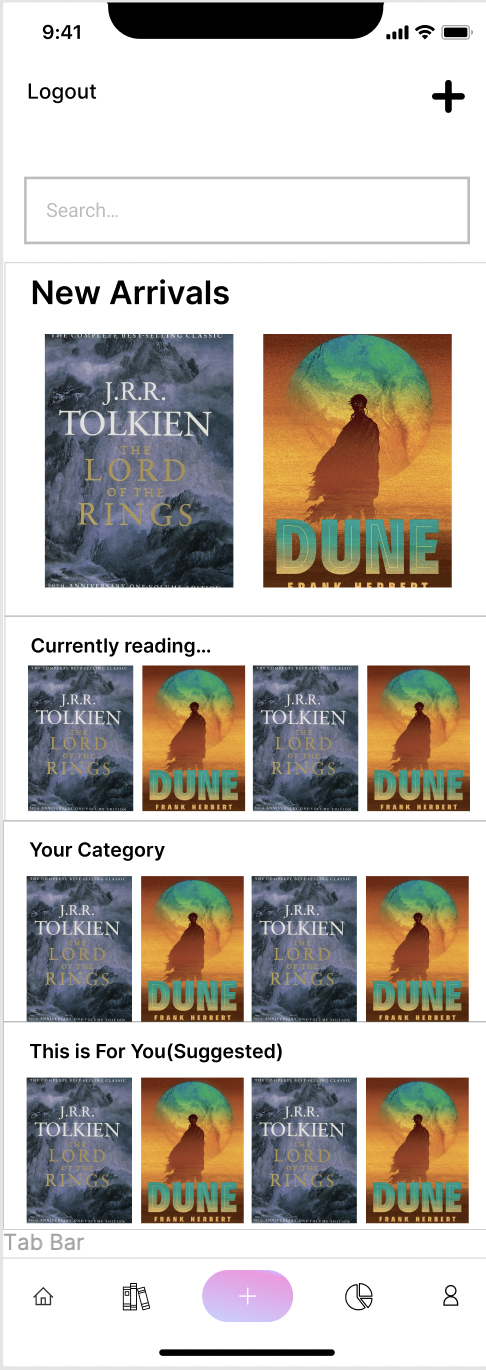
\includegraphics[width=3cm]{Ressources/Specifications/mainpage.png}
    \caption{Main page}
    \label{fig:mainpage}
\end{figure}

\subsection{User Account}
The user account page, as seen in Figure \ref{fig:useracc}, previews the user's personal information as well as the option to change any of the information, or delete the account entirely. At the top of the page, the user has the option to log-out of the application or to access the 'Settings' page of the application, as seen in Figure \ref{fig:settings}. \\

The settings page offers the user to customize different aspects of the application, such as a light/dark mode, language options and which notifications the user prefers to receive.


\begin{figure}[h]
    \centering
    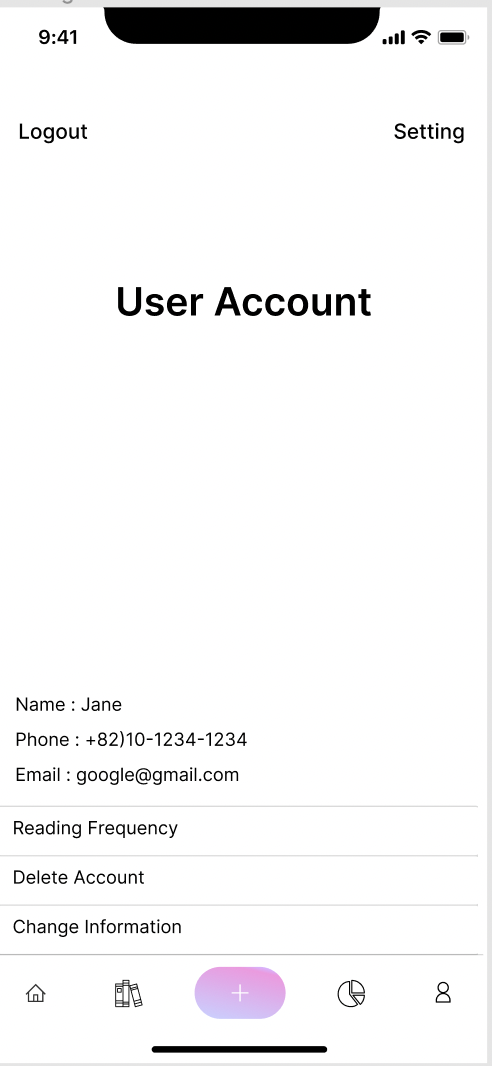
\includegraphics[width=3cm]{Ressources/Specifications/useracc.png}
    \caption{User Account page}
    \label{fig:useracc}
\end{figure}

\begin{figure}[h]
    \centering
    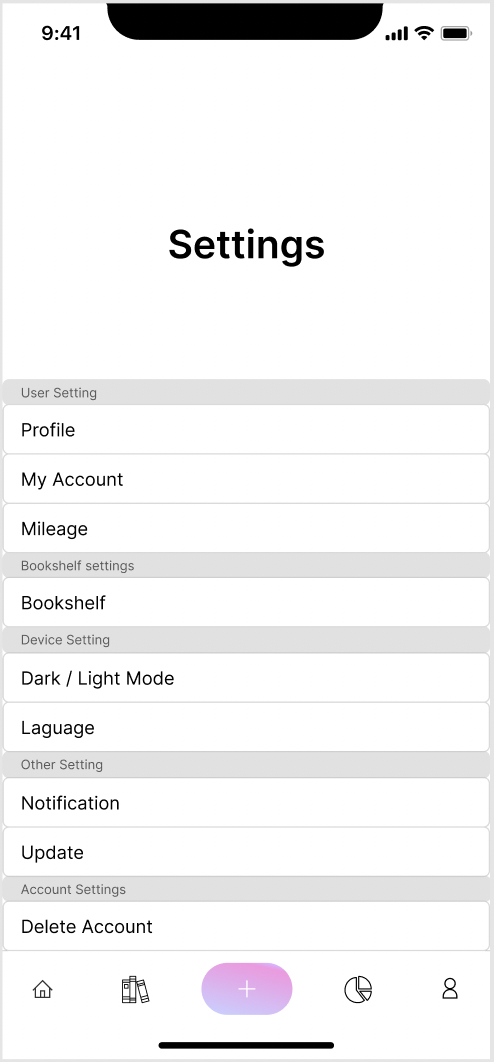
\includegraphics[width=3cm]{Ressources/Specifications/settings.png}
    \caption{Settings page}
    \label{fig:settings}
\end{figure}

\subsection{Statistics}














\begin{thebibliography}{00}
\bibitem{RFID} 
\url{https://gzandea.en.ecplaza.net/products/rfid-smart-bookshelveshf-intelligence-bookshelffile-management_3914989}

\bibitem{Smartbookshelf}
\url{https://www.red-dot.org/ko/project/smart-ai-modular-bookshelf-26628}

\bibitem{Goodreads}
\url{https://www.goodreads.com/}

\bibitem{Bookbrowse}
\url{https://www.bookbrowse.com/}

\bibitem{Storygraph}
\url{https://www.thestorygraph.com/}

\bibitem{LDM}
\url{https://drive.google.com/file/d/1qXDdPbP0vvrqVYIyJdMQ6C-DeG7IgjeZ/view?usp=sharing}

\end{thebibliography}





\end{document}